%%% CHEP 2019 protoDUNE-SP DQM evolution paper

%%%\documentclass[option]{webofc}
%%% "twocolumn" for typesetting an article in two columns format (default one column)


\documentclass{webofc}
\usepackage[varg]{txfonts}   % Web of Conferences font

%
% Put here some packages required or/and some personnal commands
%

\usepackage{xspace}
\usepackage{tabularx}

\newcommand{\pd}{protoDUNE\xspace}
\newcommand{\filesize}{8\,GB\xspace}

%%%%%%%%%%%%%%%%%%%%%%%%%%%% BEGIN %%%%%%%%%%%%%%%%%%%%%%%%%%%%%%%

\begin{document}
%
\title{Evolution of the Data Quality Monitoring and Prompt Processing System in the protoDUNE-SP experiment}


\author{
\firstname{Maxim} 
\lastname{Potekhin}\inst{1}\fnsep\thanks{\email{potekhin@bnl.gov}}, \it{on behalf of the DUNE Collaboration}
}

\institute{Brookhaven National Laboratory, Upton, NY11973, USA}


\abstract{
The DUNE Collaboration has successfully implemented and currently operates
an experimental program based at CERN which includes a beam test and an extended
cosmic ray run of two large-scale prototypes of the DUNE Far Detector.
The volume of data collected by the protoDUNE-SP (the single-phase
Liquid Argon TPC prototype) amounts to $\sim$3PB and the sustained rate
of data sent to mass storage is O(100) MB/s.  A fraction of the data stream
is captured by the protoDUNE Prompt Processing System (p3s) which is optimized
for continuous low-latency calculation of the vital detector metrics and various graphics
including event displays. This system is the platform for Data Quality Monitoring in protoDUNE-SP
and has served a crucial role throughout the life cycle of the experiment.
We present our experience in operating the system in the CERN environment, along
with work currently underway to make the system more scalable, resilient and
to simplify system recovery procedures in preparation for the second beam
run of protoDUNE-SP foreseen after the Long Shutdown 2 of the LHC.
}
%
\maketitle
%
\section{Introduction}

\label{sec:intro}
The \pd-SP experiment is designed to study a large-scale prototype of the single-phase version of
the Liquid Argon Time Projection Chamber (LArTPC) which will eventually become one of
the principal elements of the DUNE apparatus to be constructed at the Sanford Underground
Research Facility \cite{cdrVol1, cdrVol4}. The prototype (CERN designation NP04) is located
in the CERN North Experimental Hall and is tested utilizing a dedicated beam line from the CERN SPS
accelerator complex. The run plan also includes a large number of cosmic ray triggers.
Commisioning of the detector took place in September of 2018.


\section{Section title}
\label{sec-1}
For bibliography use \cite{RefJ}
\subsection{Subsection title}
\label{sec-2}
Don't forget to give each section, subsection, subsubsection, and
paragraph a unique label (see Sect.~\ref{sec-1}).

For one-column wide figures use syntax of figure~\ref{fig-1}
\begin{figure}[h]
% Use the relevant command for your figure-insertion program
% to insert the figure file.
\centering
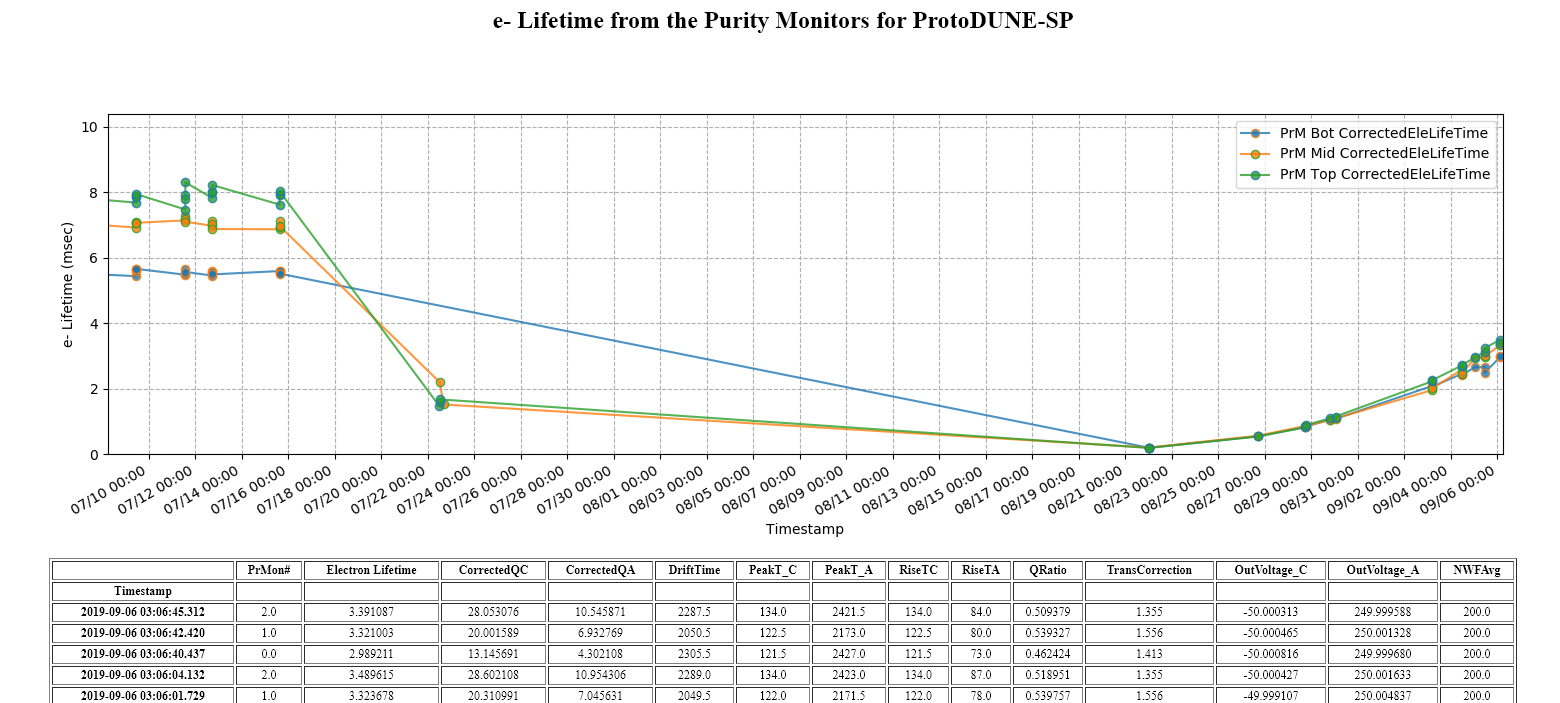
\includegraphics[width=1cm,clip]{figures/dqm_purmon_20190910_1.png}
\caption{Please write your figure caption here}
\label{fig-1}       % Give a unique label
\end{figure}

For two-column wide figures use syntax of figure~\ref{fig-2}
\begin{figure*}
\centering
% Use the relevant command for your figure-insertion program
% to insert the figure file. See example above.
% If not, use
\vspace*{5cm}       % Give the correct figure height in cm
\caption{Please write your figure caption here}
\label{fig-2}       % Give a unique label
\end{figure*}

For figure with sidecaption legend use syntax of figure
\begin{figure}
% Use the relevant command for your figure-insertion program
% to insert the figure file.
\centering
\sidecaption
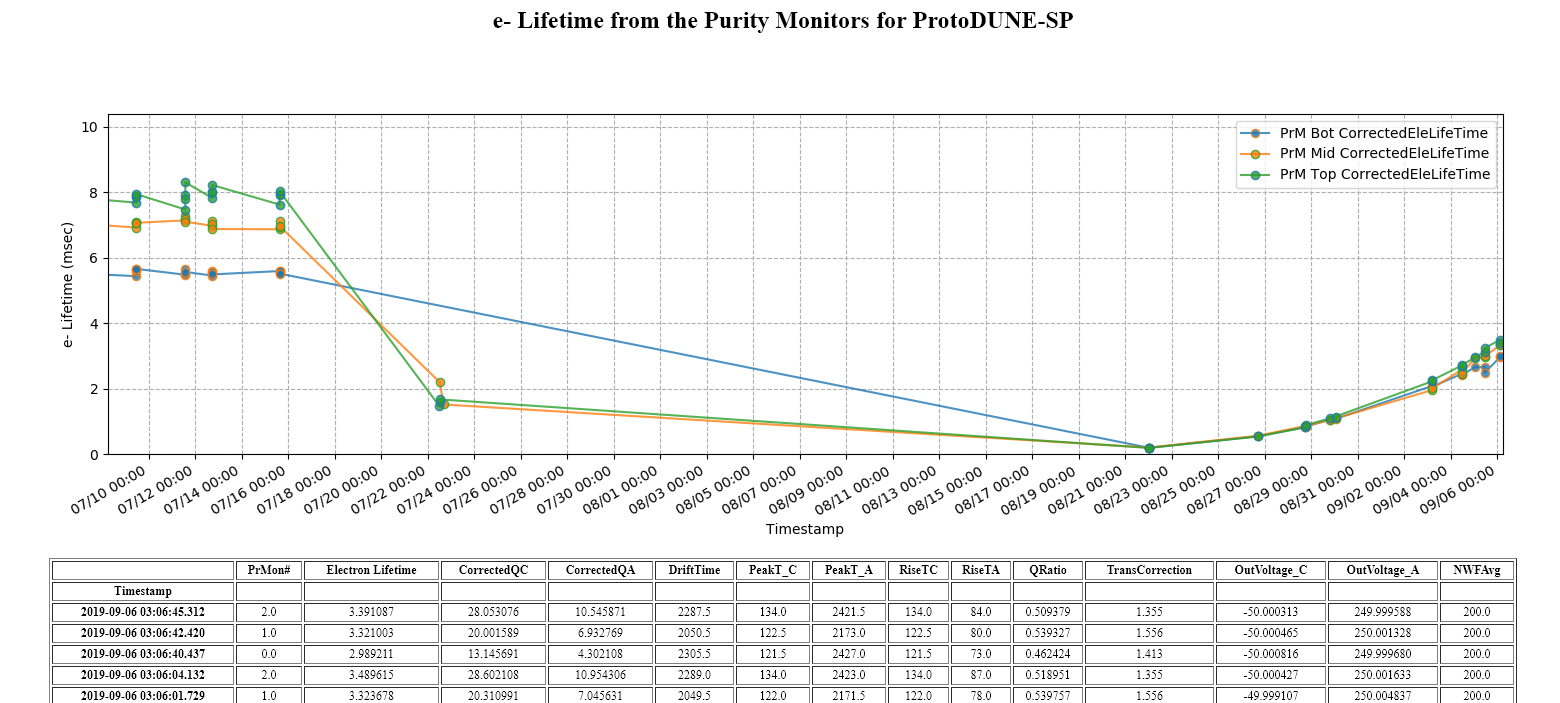
\includegraphics[width=5cm,clip]{figures/dqm_purmon_20190910_1.png}
\caption{Please write your figure caption here}
\label{fig-3}       % Give a unique label
\end{figure}

For tables use syntax in table~\ref{tab-1}.
\begin{table}
\centering
\caption{Please write your table caption here}
\label{tab-1}       % Give a unique label
% For LaTeX tables you can use
\begin{tabular}{lll}
\hline
first & second & third  \\\hline
number & number & number \\
number & number & number \\\hline
\end{tabular}
% Or use
\vspace*{5cm}  % with the correct table height
\end{table}

\begin{thebibliography}{99}

\bibitem{cdrVol1}
R. Acciarri et al.
\emph{Long-Baseline Neutrino Facility (LBNF) and Deep Underground Neutrino Experiment (DUNE) Conceptual Design Report Volume 1: The LBNF and DUNE Projects}.\\ ~e-Print: arXiv:\textbf{1601.05471}
 %DUNE CDR Vol 1 -- The LBNF and DUNE Projects.~e-Print: arXiv:1601.05471
%\url{http://arxiv.org/abs/1601.05471}

\bibitem{cdrVol4}
R. Acciarri et al.
\emph{Long-Baseline Neutrino Facility (LBNF) and Deep Underground Neutrino Experiment (DUNE) Conceptual Design Report, Volume 4: The DUNE Detectors at LBNF}.\\~e-Print: arXiv:\textbf{1601.02984}
%\url{http://arxiv.org/abs/1601.02984}

\bibitem{eps} M.Potekhin et al. \emph{The protoDUNE-SP experiment and its prompt
processing system}. Proceedings of Science (EPS-HEP2017) 513

%\bibitem{uboone}
%B. Jones et al.  \emph{The Status of the MicroBooNE Experiment.~J. Phys.: Conf. Series.} Vol.\textbf{408}. IOP Publishing, 2013,
%doi:10.1088/1742-6596/408/1/012028


\bibitem{sam}
R. A. Illingworth \emph{A data handling system for modern and future Fermilab experiments.~J. Phys.: Conf. Series.} Vol.\textbf{513}. IOP Publishing, 2014,
doi:10.1088/1742-6596/513/3/032045

\bibitem{fts}
A. Norman \emph{The Fermilab File Transfer System}.~e-Print: FNAL CD-DocDB-5412

\bibitem{castoreos}
 L. Mascetti et al. \emph{Disk storage at CERN.~J. Phys.: Conf. Series.} Vol.\textbf{664}. IOP Publishing, 2015,
doi:10.1088/1742-6596/664/4/042035

\bibitem{eos_role}
S. Fuess et al. \emph{Design of the protoDUNE raw data management
infrastructure.~J. Phys.: Conf. Series.} Vol.\textbf{898}. IOP Publishing, 2017,
doi:10.1088/1742-6596/898/6/062036

%\bibitem{xrootd}
%L. Bauerdick et al. \emph{Using Xrootd to Federate Regional Storage.~J. Phys.: Conf. Series.} Vol.\textbf{396}. IOP Publishing, 2012,
%doi:10.1088/1742-6596/396/4/042009

\bibitem{panda}
T. Maeno et al. \emph{Overview of ATLAS PanDA Workload Management.~J. Phys.: Conf. Series.} Vol.\textbf{331}. IOP Publishing, 2011,
doi:10.1088/1742-6596/331/7/072024



\bibitem{dirac}
A. Casajus et al.  \emph{DIRAC Pilot Framework and the DIRAC
Workload Management System.~J. Phys.: Conf. Series.} Vol.\textbf{219}. IOP Publishing, 2010,
doi:10.1088/1742-6596/219/6/062049

\bibitem{django}
N. George \emph{Mastering Django: Core. The Complete Guide to Django 1.8 LTS}~ GNW Independent Publishing, ISBN: 099461683X


\end{thebibliography}




\end{document}

% end of file template.tex

<div id='footer'><table width='100%'><tr><td class='right'><a href='http://fusioninventory.org/'><span class='copyright'>FusionInventory 9.1+1.0 | copyleft <img src='/glpi/plugins/fusioninventory/pics/copyleft.png'/>  2010-2016 by FusionInventory Team</span></a></td></tr></table></div>